%%%%%%%%%%%%%%%%%%%% Chapter 3
\chapter{Lasso Gripper: Design, Analysis, and Experiments}

This chapter introduces the Lasso Gripper as the first mechanism embodiment of the thesis. The design investigates how a tendon-driven system can use a flexible tensile element not only for force transmission but also for adaptive grasp formation. Conventional rigid grippers often struggle when the target object exceeds the maximum opening width or presents soft, fragile, or highly variable geometry. In such cases, increasing gripping force alone can raise the risk of slippage, deformation, or damage.

To address this limitation, the Lasso Gripper is proposed as an integrated mechatronic system optimized for adaptive capture, high-speed operation, and distributed contact through a controllable string loop. The following sections describe its mechanical architecture, the dedicated mechanisms for string deployment and retraction, and the control structure that enables its dynamic grasping behavior. The chapter establishes the mechanism principles that are later translated into the handheld surgical instrument presented in this thesis.
% ------------------------- 2.1 Overall Structure -------------------------
\section{Design and Principle}

\begin{figure}[htbp]
\centering
\begin{tabular}{cc}
\begin{minipage}[t]{0.9\textwidth}
\centering
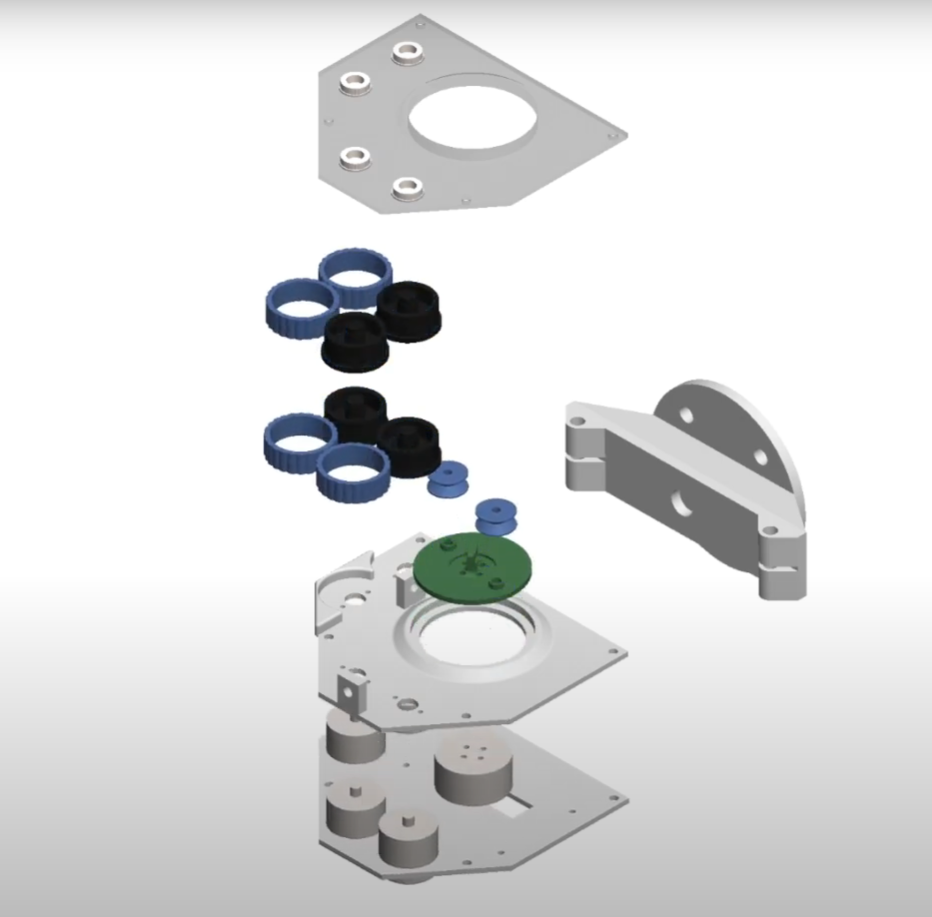
\includegraphics[width=1\columnwidth]{Figures/overall_img.png}
\caption{The SolidWorks designed hardware of the proposed gripper}
\end{minipage}
\end{tabular}
\end{figure}

Lasso Gripper comprises several crucial elements, including the robotic arm, controller, power supply, and communication interfaces. The robotic arm is engineered to provide the necessary degrees of freedom and precision required for accurate positioning and manipulation. The controller is responsible for managing the gripper's operations, processing sensor inputs, and executing the gripping actions. It employs advanced algorithms to ensure optimal performance. The power supply guarantees consistent electrical energy to all components, while communication interfaces enable seamless data exchange between the gripper and the central control system, ensuring synchronized operations.

\begin{figure}[htbp]
\centering
\begin{tabular}{cc}
\begin{minipage}[t]{0.9\textwidth}
\centering
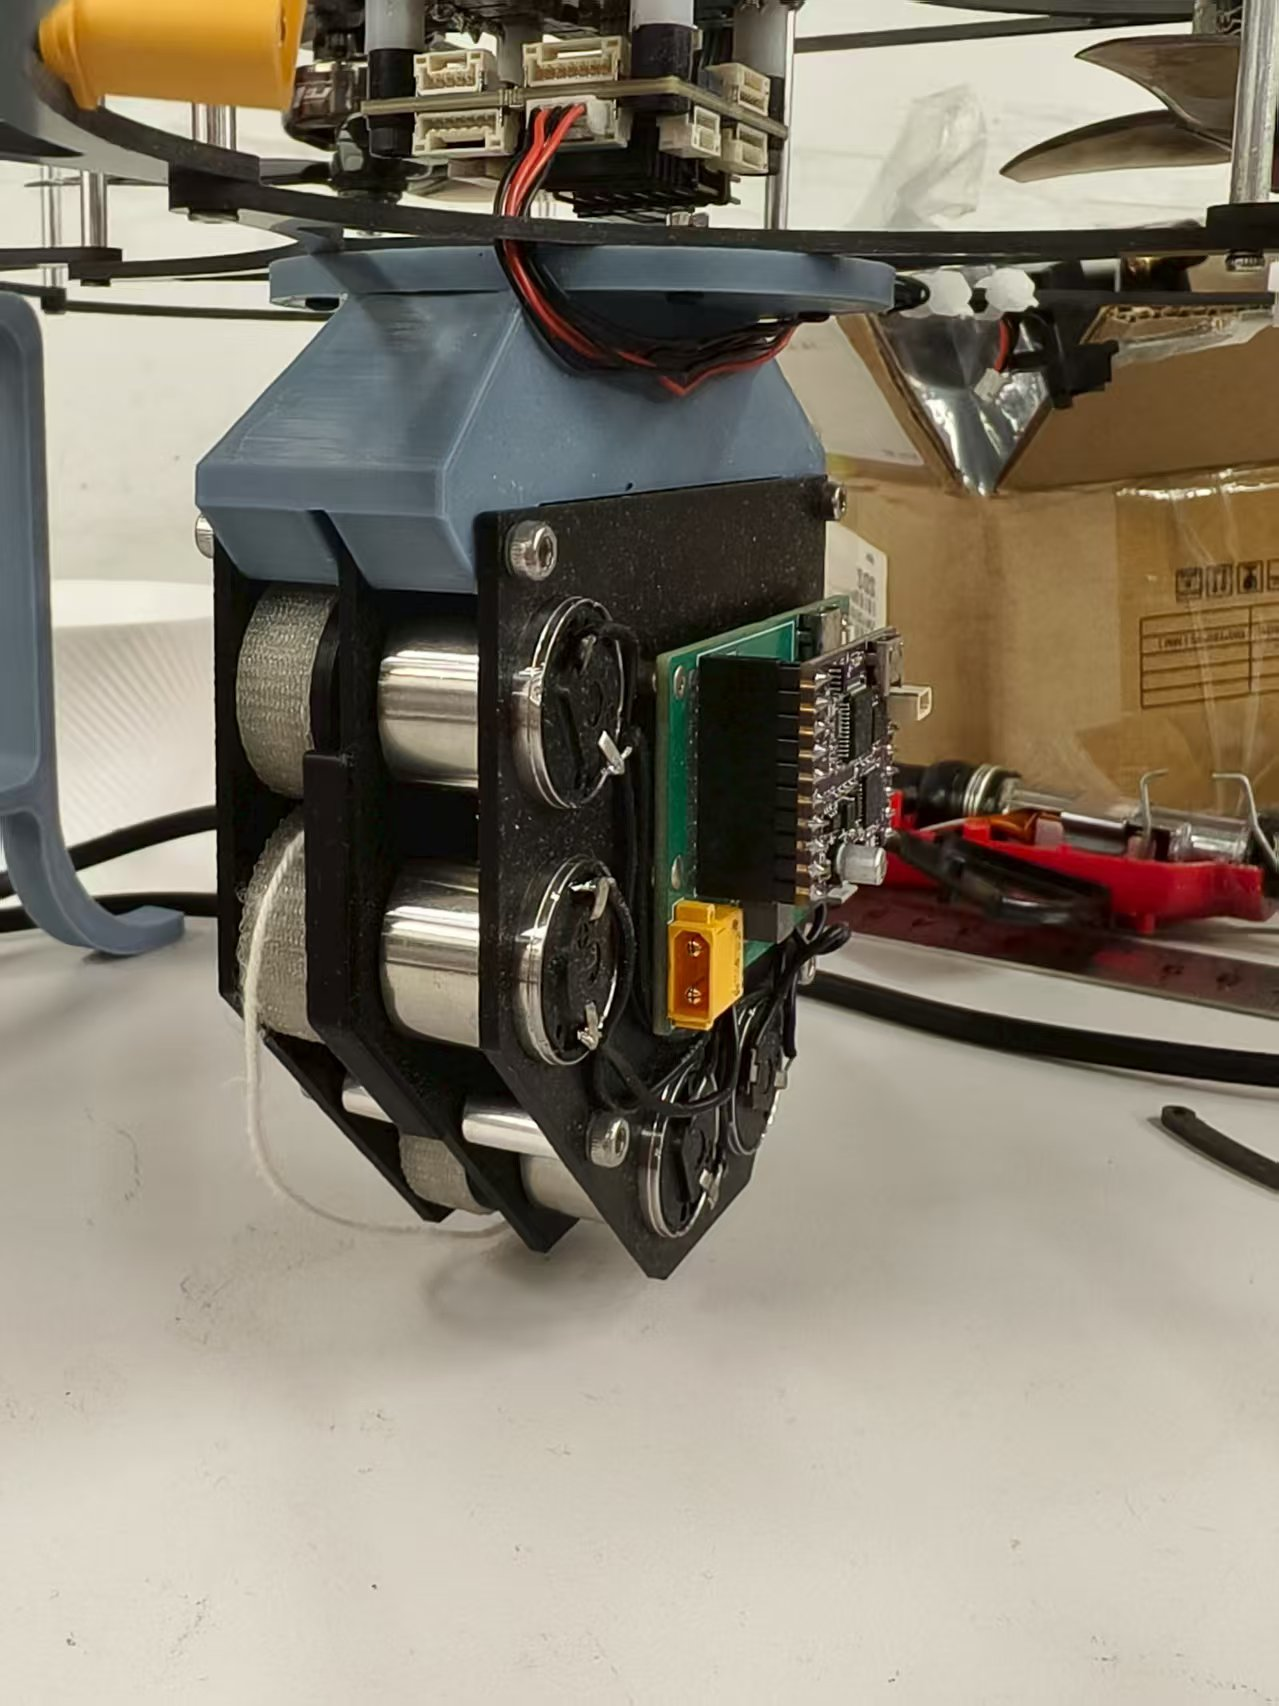
\includegraphics[width=1\columnwidth]{Figures/system_overview.jpg}
\caption{The proposed gripper connected with an ESP32 controller, motor electronic speed controller.}
\end{minipage}
\end{tabular}
\end{figure}



% ------------------------- 2.2 String Shooting and Retraction Mechanism -------------------------
\subsection{String Shooting and Retraction Mechanism}

The string shooting and retraction mechanism is a defining feature of Lasso Gripper, enabling it to perform complex gripping tasks with high efficiency. The mechanism comprises multiple components working in unison to achieve precise control over the string's movement.

The propulsion of the string is achieved through two pairs of friction wheels. These wheels are designed with high-friction surfaces to grip the string effectively. The wheels are driven by coreless motors with high speed so that the required rotational speeds for rapid string extrusion can be achieved\cite{murata2024elastic}.

During the string shooting phase, both pairs of friction wheels rotate in the same direction, propelling the string forward through a guided track. This track is meticulously designed to ensure the string forms a loop within the desired dimensions and shape. Sensors along the track monitor the string's position and velocity, providing real-time feedback to the controller.

\begin{figure}[htbp]
\centering
\begin{tabular}{cc}
\begin{minipage}[t]{0.9\textwidth}
\centering
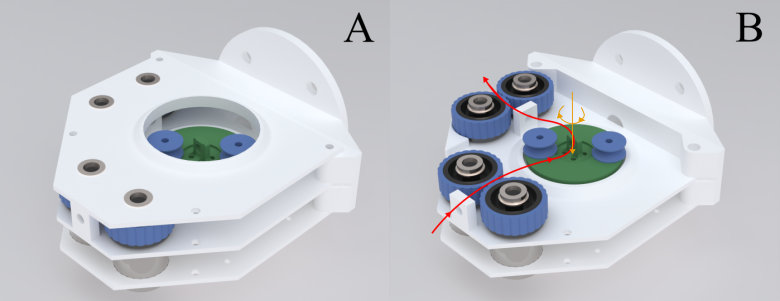
\includegraphics[width=1.0\columnwidth]{Figures/Figure11.png}
\caption{The friction wheels and the retraction mechanism driving motors are highlighted for illustration.}
\end{minipage}
\end{tabular}
\end{figure}

When retraction is required, the mechanism undergoes a coordinated sequence of actions. The rear pair of friction wheels maintains its rotational speed, continuing to pull the string inwards. Simultaneously, the front pair of wheels reverses direction, creating a counterforce that pulls the string loop into the space between the two pairs of wheels. This space is precisely designed to accommodate the retracted string without entanglement.

Within this confined space, a spool mechanism is designed. The spool is equipped with a rotational motor that winds the string onto itself, storing it neatly for future use. The tension exerted on the string during retraction is carefully controlled by a force feedback sensor located on the spool's axle. This sensor monitors the tension and adjusts the motor's torque to ensure that the object is gripped securely without applying excessive force that could cause damage.

\subsection{The ESP32 Main Controller for Lasso Gripper}

The ESP32 Main Controller serves as the central hub for managing the operations of Lasso Gripper. The ESP32 integrated Wi-Fi and Bluetooth capabilities, provides both the computational power and connectivity required for the gripper's complex functions.
\begin{figure}[htbp]
\centering
\begin{tabular}{cc}
\begin{minipage}[t]{0.5\textwidth}
\centering
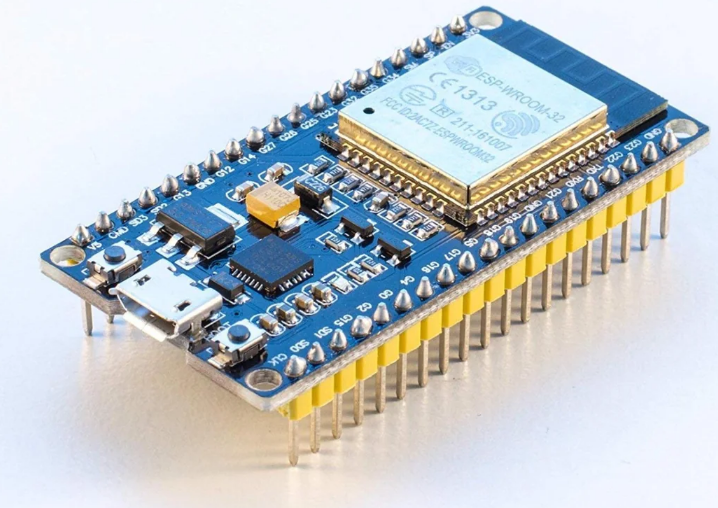
\includegraphics[width=1.0\columnwidth]{Figures/esp32.png}
\caption{The ESP32 controller used in the proposed Lasso Gripper.}
\end{minipage}
\end{tabular}
\end{figure}
At the heart of the ESP32 Main Controller is its dual-core processor, which efficiently handles multiple tasks simultaneously. This includes real-time processing of sensor data, executing gripping algorithms, and maintaining communication with external devices. The controller interfaces with various sensors, such as force sensors and motion trackers, to gather critical data on gripping forces, positioning accuracy, and object integrity.

The ESP32's GPIO (General Purpose Input/Output) pins are utilized to control the retraction modules that adjust the grasping force of the lasso, ensuring precise manipulation of objects. Additionally, the controller's PWM (Pulse Width Modulation) capabilities allow for fine-tuned control of the friction wheels.

The integrated Wi-Fi and Bluetooth features of the ESP32 facilitate seamless communication with a upper computer for target recognition and grasping planning. This connectivity also allows for remote monitoring and control, data logging, and integration with broader automation systems.

\section{Implications for Tendon-Driven Mechanisms and Medical Devices}

The Lasso Gripper work provides several mechanism-level insights that generalise beyond the specific prototype. First, the principle of using a flexible tensile element to create an adaptive capture region suggests new ways to trade capture range for control complexity. Second, differential and proximal actuation patterns enable low distal mass while still producing multi-degree-of-freedom effects at the end-effector; this trade-off is central to designing hand-held tools and remote manipulators. Third, performance metrics such as capture probability, peak tensile load, retraction dynamics, and hysteresis in the cable path form a compact evaluation set that is applicable to other tendon-driven designs.

These insights motivated the subsequent handheld surgical instrument presented in this thesis: the instrument intentionally reuses the same tendon-driven design philosophy and control principles, but applies them to the clinical constraints of minimally invasive surgery (low profile, ergonomic balance, safety and sterilizability). The following chapter therefore uses the Lasso Gripper both as a technical proof-of-concept and as a source of formalised mechanism design rules.
